
% Initial Template by Arnau, adapted to needs by Tobia:

\documentclass[.08pt,t]{beamer}

\mode<presentation> {

\usetheme{Boadilla}

% As well as themes, the Beamer class has a number of color themes
% for any slide theme. Uncomment each of these in turn to see how it
% changes the colors of your current slide theme.

% \usecolortheme{albatross}
%\usecolortheme{beaver}
%\usecolortheme{beetle}
%\usecolortheme{crane}
% \usecolortheme{dolphin}
%\usecolortheme{dove}
% \usecolortheme{fly}
% \usecolortheme{lily}
%\usecolortheme{orchid}
%\usecolortheme{rose}
%\usecolortheme{seagull}
\usecolortheme{seahorse}  % The them I usually use, because it resembles the PSI template.
% \usecolortheme{whale}
% \usecolortheme{wolverine}

%\setbeamertemplate{footline} % To remove the footer line in all slides uncomment this line
% \setbeamertemplate{footline}[page number] % To replace the footer line in all slides with a simple slide count uncomment this line
}

% Disable shadowed blocks and rounded corners in blocks
\setbeamertemplate{blocks}[rounded][shadow=false, rounded=false]

% Custom bullet-points for the whole document
\setbeamertemplate{itemize items}[circle]

% Use regular font for math mode text
\renewcommand\mathfamilydefault{\rmdefault}

\setbeamertemplate{sections/subsections in toc}[sections numbered]  % Controls style of number in the table of contents.

\makeatletter
\setbeamertemplate{footline}{
  \leavevmode%
  \hbox{\fontsize{5}{7}\selectfont%
  \begin{beamercolorbox}[wd=.333333\paperwidth,ht=2.8ex,dp=1ex,left]{author in head/foot}%
    \usebeamerfont{author in head/foot}\hspace*{2ex}\insertshortauthor\expandafter\beamer@ifempty\expandafter{\beamer@shortinstitute}{}{~~(\insertshortinstitute)}
  \end{beamercolorbox}%
  \begin{beamercolorbox}[wd=.333333\paperwidth,ht=2.8ex,dp=1ex,center]{title in head/foot}%
    \usebeamerfont{section in head/foot}\insertsection
  \end{beamercolorbox}%
  \begin{beamercolorbox}[wd=.333333\paperwidth,ht=2.8ex,dp=1ex,right]{date in head/foot}%
    \usebeamerfont{date in head/foot}\insertshortdate{}\hspace*{4em}
    \insertframenumber{} / \inserttotalframenumber\hspace*{2ex}
  \end{beamercolorbox}}%
  \vskip0pt%
}
\makeatother

\setbeamertemplate{navigation symbols}{}  % Remove navigation symbols
\setbeamersize{text margin left=1cm,text margin right=1cm}

\setbeamertemplate{caption}[numbered]

% Insert title slide at beginning of each section
\AtBeginSection[]{
  \begin{frame}
  \vfill
  \centering
  \begin{beamercolorbox}[sep=8pt,center,shadow=False,rounded=true]{title}
      \usebeamerfont{title}\insertsectionhead\par%
  \end{beamercolorbox}
  \vfill
  \end{frame}
}

% \newenvironment<>{greyBlock}{%
%     \setbeamercolor{block title}{use=structure,fg=white,bg=\usebeamercolor[fg]{structure}}%
%     \setbeamercolor{block body}{use=structure,fg=black,bg=gray!20!white}%
%     \setbeamerfont{block body}{size=\footnotesize}%
% \begin{beamercolorbox}
%     \begin{block}{}%
%     }{%
%     \end{block}%
% }

% Set font size for regular blocks for whole documents
\setbeamerfont{block title}{size=\normalsize}
\setbeamerfont{block body}{size=\small}

\newenvironment<>{definitionBlock}{%
    \setbeamercolor{block title}{use=structure,fg=white,bg=gray!50!black}%
    \setbeamercolor{block body}{use=structure,fg=black,bg=gray!20!white}%
    \setbeamerfont{block body}{size=\footnotesize}%
    \begin{block}{}%
    }{%
    \end{block}%
}

% Bibliography
% \makeatletter\@ifpackageloaded{biblatex}{\addbibresource{references.bib}}{\bibliography{references}}\makeatother

\usepackage{amsmath}
\usepackage{amssymb}
\usepackage{amsthm}
\usepackage{amsfonts}
\usepackage{enumitem}
\usepackage{fancyhdr}
\usepackage[a4paper]{geometry}
\usepackage{listings}
\usepackage{placeins}
\usepackage{siunitx}
\usepackage{tikz}

\usepackage[lowercase]{theoremref}
\usepackage{graphicx}
\usepackage{tabularx}
\usepackage{caption}
\usepackage{subcaption}
\usepackage{verbatim}
\usepackage{verbatimbox}
\usepackage{xcolor, colortbl}
\usepackage[hidelinks]{hyperref}
\usepackage{pdfpages}
\usepackage{physics}
\usepackage[titletoc,title]{appendix}
\usepackage{booktabs}
\usepackage{cleveref}
\usepackage{float}
\usepackage{todonotes}
\usepackage[export]{adjustbox}
\usepackage[acronym]{glossaries-extra}
\usepackage{doi}

% Algorithm listings
\usepackage{algorithm}
\usepackage{algpseudocode}
\usepackage{pifont}

% Code listings
\usepackage{minted}

\usepackage{multicol}
\usepackage{multirow}

\usetikzlibrary{shapes,arrows, matrix, decorations.pathreplacing}%fit

%\urlstyle{same} % 09.09.2015, http://latex-community.org/forum/viewtopic.php?f=50&t=4191
% \bibliographystyle{ieeetr}
\bibliographystyle{IEEEtran}

\newtheorem{theorem}{Theorem} %13.05.2015, https://www.sharelatex.com/learn/Theorems_and_proofs#Proofs

%\newcommand{\ref}[1] {Fig.\ \ref{#1}}
\newcommand{\lstref}[1] {Lst.\ \ref{#1}}
\newcommand{\tabref}[1] {Tab.\ \ref{#1}}
\newcommand{\secref}[1] {Sec.\ \ref{#1}}
\newcommand{\outref}[1] {Output \ref{#1}}
\newcommand{\enumref}[1] {Appendix \ref{#1}}
\newtheorem{mydef}{Definition}
% \newcommand{\eqsref}[1] {Eq.\ \ref{#1}}

\lstdefinestyle{MyLstDesign}{
    basicstyle=\scriptsize\ttfamily,
    captionpos=b,
    showspaces=false,
    showstringspaces=false,
    breaklines=true,
    frame=L,
    xleftmargin=0.65cm,
    numbers=left,
    commentstyle=\itshape\color{red},
    keywordstyle=\color{black!50!green}
}

% 06.09.2015, http://stackoverflow.com/questions/2709898/change-list-of-listings-text
% \renewcommand{\lstlistingname}{List of Listings}
\renewcommand{\lstlistlistingname}{List of Listings}

% Command for bold symbols (Vector and Matrix notation)
\newcommand{\vect}[1]{\boldsymbol{#1}}
\newcommand{\bs}[1]{\boldsymbol{#1}}
\newcommand{\uuline}[1]{\underline{\underline{#1}}}
\newcommand{\matr}[1]{\uuline{#1}}

% Vacuum permitivity
\newcommand{\vp}{\varepsilon_0}

% Normalized x-emittance
\newcommand{\eps}{\varepsilon_{x}}
\newcommand{\neps}{\varepsilon_{x,n}}

% Operators in separated phase space
\newcommand{\posNabla}{\nabla_{\vect r}}
\newcommand{\velNabla}{\nabla_{\vect v}}
\newcommand{\fdVelNabla}{\nabla_{\vect v}^{\text{fd}}}
\newcommand{\spVelNabla}{\nabla_{\vect v}^{\text{sp}}}
\newcommand{\fdPosNabla}{\nabla_{\vect r}^{\text{fd}}}
\newcommand{\spPosNabla}{\nabla_{\vect r}^{\text{sp}}}

\newcommand{\velHess}{\matr H_{\vect v}}
\newcommand{\fdVelHess}{\matr H_{\vect v}^{\text{fd}}}
\newcommand{\spVelHess}{\matr H_{\vect v}^{\text{sp}}}

% Spacing between equations
\newcommand{\eqVspace}{\\[7pt]}

% Moment brackets
\newcommand{\bracket}[1]{\langle {#1} \rangle}

% Method names
\newcommand{\pcubem}{P\textsuperscript{3}M\ }


\title[\today]{The Langevin Approach to Discretize the Collision Operator}


\author{Tobia Claglüna}
\institute[LSM, PSI]{
    AMAS Group, LSM\\ % Your institution for the title page.
}
\date{\today}
\def \myEmail {tobia.clagluena@psi.ch}

% \beamerdefaultoverlayspecification{<+->}

\begin{document}
\def\vfilll{\vskip 0pt plus 1filll minus 0pt }
\begin{frame}
  % Title page image:
  \vspace{0.3cm}
  \begin{adjustbox}{width=\paperwidth, center}
    \begin{tikzpicture}
      \centering
      \filldraw[fill=lightgray!40!white, draw = none] (0,0) rectangle (3.3,0.5\textheight);
      % Logos:
      \node[anchor=south west,inner sep=0] at (0.4,3.4)
           {
\includegraphics[width=2.5cm]{logos/PSI.pdf}};
      \node[anchor=south west,inner sep=0] at (0.5,1.8)
           {
\includegraphics[width=2.4cm]{logos/eth_logo_kurz_pos-eps-converted-to.pdf}};
    \end{tikzpicture}
    \begin{tikzpicture}
      \node (heli) [anchor=south west,inner sep=0] at (0,0)
            {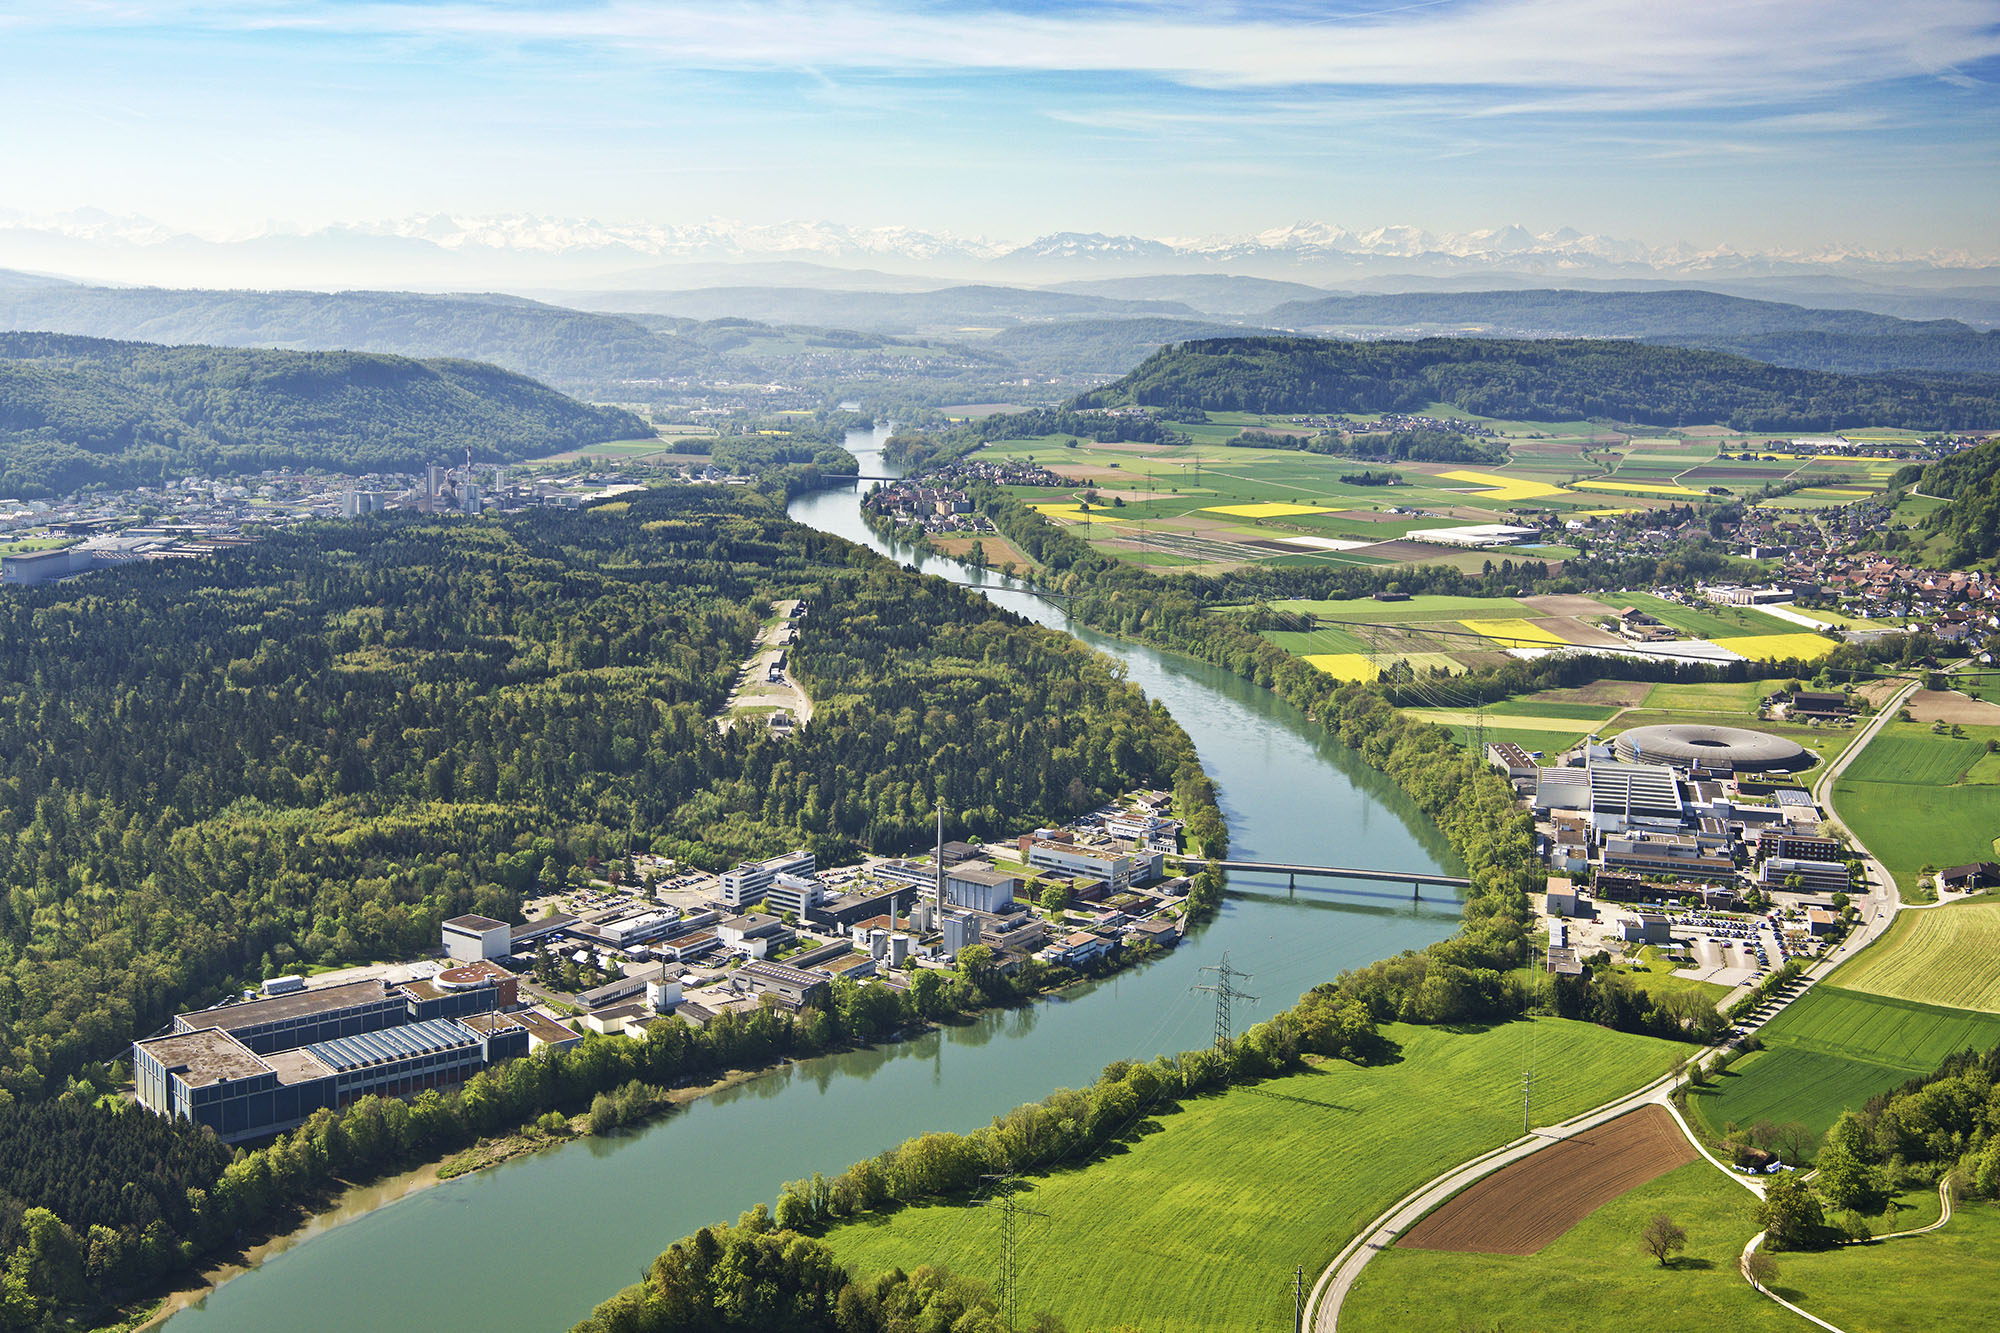
\includegraphics[height=0.5\textheight]{logos/PSI_helicopter}};
      \node [anchor=south west, inner sep = 1,fill=white, opacity=0.8] at (3.5, 0.0)
            {\tiny WIR SCHAFFEN WISSEN – HEUTE FÜR MORGEN};
    \end{tikzpicture}
    \begin{tikzpicture}
      \filldraw[fill=lightgray!40!white, draw = none] (0,0) rectangle (1,0.5\textheight);
    \end{tikzpicture}
  \end{adjustbox}
  \vspace{0.1cm}\\
  {\usebeamerfont{subtitle} \footnotesize \insertauthor\, ::  \insertinstitute}
  \vfilll
  \vspace{0.4cm}
  {\usebeamerfont{title} \Large \inserttitle}\\
  \vfilll
  \vspace{0.1cm}
  {\usebeamerfont{subtitle} {\large Master's Thesis Presentation}}\\
  \vfilll
  \vspace{0.2cm}
  {\usebeamerfont{subtitle} \footnotesize \insertdate}\\
  \null\hfill\tiny Contact: \url{\myEmail}
\end{frame}


\begin{frame}{Outline}
    \setcounter{tocdepth}{1}
  \tableofcontents
\end{frame}

\section{Motivation}

% \begin{frame}{Mismatch between Simulation and Experiment}
%     \begin{itemize}
%         \item I implemented a solver to simulate nonneutral cold plasmas (low kinetic energy, high
%         potential). Potential E gets transferred to Kinetic energy via collisions
%         \item FELs are machines in which plasma reaches states where exactly this happens.
%         \item Applications: structure of proteins / or crystalline matter
%         \item Accelerated particle bunches emit short radiation pulses at very short wavelengths
%         \item Problem arises with a phenomenon called "intrabeam scattering" widening the beam as
%             shown by Prat
%         \item Energy spread limits compression
%         \item Instead of modeling binary collisions, we use explore a stochastic approach based on
%             a formulation of the Langevin equation
%         \item Collision operator
%     \end{itemize}
% \end{frame}

\begin{frame}{Motivation}
    \begin{block}{Plasma dynamics in Free Electron Lasers (FELs)}
    \begin{itemize}
        \itemVspace
        \item Accelerated particle bunches emit radiation after passing through undulators
        \item Particle bunches emit radiation at very short wave lengths (many possible
            applications) 
    \end{itemize}
    \end{block}

    \vspace{0.7mm}
    \pause

    \begin{block}{Problem}
    \begin{itemize}
        \itemVspace
        \item Experiment-Simulation mismatch on energy spread (\cite{prat2022energy})
        \item Energy spread limits bunch compression % (lower bound on emitted wave length)
        \item Intrabeam Scattering widens beam
        \item Existing method for modeling collisions is too expensive (\cite{Hockney2021})
    \end{itemize}
    \end{block}

    \vspace{0.7mm}
    \pause

    \begin{block}{Outlook}
        \begin{itemize}
            \itemVspace
            \item Stochastic Ansatz for modeling collisions (Langevin)
            \item Better computational complexity
            \item Run solver on an analytical and a real-world test case
        \end{itemize}
    \end{block}

\end{frame}

\section{Theory}

\begin{frame}{Notation}

\begin{table}[h]
    \centering
    \caption{Notation used throughout the presentation.}
    \begin{tabularx}{0.78\textwidth}{l l}
        \toprule
        Symbol & Definition \\
        \midrule
        $\vect a$ & Vector quantity $\in \mathbb R^3$ \tabVspace
        $\vect a_i$ & Vector component at index $i$ \tabVspace
        $\lVert \vect b \rVert_2 = \sqrt{\sum_i \vert b_i \vert^2}$ & $L^2$-norm \tabVspace
        $\matr B$ & Tensor quantity $\in \mathbb R^{3\times 3}$ \tabVspace
        $\matr B_{i,j}$ & Tensor component at index $(i,j)$ \tabVspace
        $\matr C : \matr E$ & $\sum_{i,j} \matr C_{i,j} \matr E_{i,j}$ \tabVspace
        $\velNabla$ & Gradient operator acting on velocity space \tabVspace
        $\matr H_{\vect v}$ & Hessian operator acting on velocity space \\
        \bottomrule
    \end{tabularx}
    \label{table:nomenclature}
\end{table}

\end{frame}

\begin{frame}{Vlasov-Poisson Equation}
%     \begin{itemize}
%         \item Define system dynamics with phase space description (allows resolving small-scale
%             structures appearing far from thermal equilibrium in the plasma)
%         \item f_k is a function based on dirac deltas which describes where the particles lie in
%         phase space
%         \item Evolution of phase space is described by a continuity equation as follows (see Eq. 2.9
%             in report)
%         \item Introduce r.h.s. collisional term (captures interactions between particles, and is
%         needed to proper relaxation of the system to thermal equilibrium)
%         \item Together with Maxwell's equation we introduce interactions with external and
%         electric self-fields via an electrostatic assumption. Resulting Vlasov-Poisson (state chosen simplifications
%     \end{itemize}

   \only<1->
   \begin{block}{Phase Space Definition}
    \begin{equation}
        f(\vect r, \vect v, t) = \frac{1}{\Delta \vect r \Delta \vect v} \int_{\Delta \vect r} d\vect r \int_{\Delta
        \vect v} d\vect v f_K
        \label{eq:phaseSpaceDensity}
    \end{equation}
   \end{block}

   \pause
   \begin{block}{Vlasov-Poisson Equation}
       \begin{equation}
           \label{eq:VlasovPoissonEquation}
           \left\{  
               \begin{aligned}
                   \frac{\partial f}{\partial t} + \vect v \cdot \frac{\partial f}{\partial \vect r} +
                   \frac{\vect F}{m} \frac{\partial f}{\partial \vect v} &= \left( \frac{\partial f}{\partial t}
                   \right)_{\text{coll}}, \eqVspace
                   \pause
                       \posNabla^2 \phi(\vect r) &= - \frac{\rho(\vect r)}{\epsilon_0}.
                   \end{aligned}
               \right.
           \end{equation}
       \end{block}

       \pause

       \vspace{0.8mm}
       \begin{center}
               \large
           \item $\boldsymbol \rightarrow$ How do we determine the r.h.s. $\left( \frac{\partial f}{\partial t}
                   \right)_{\text{coll}}$?
       \end{center}
\end{frame}

\begin{frame}{Scattering in the center of mass frame}
    % \begin{itemize}
    %     \item List facts regarding these collisions in  the center-of-mass frame:
    %         \begin{itemize}
    %             \item Majority of interactions happen at large impact parameters
    %             \item Individual collisions are weak compared to thermal energy of the system
    %             \item Time scale at which such simultaneous collisions are experienced by the test
    %                 particle larger than the individual collision time $\tau_c$ (show inequality Eq.
    %                 2.14) $\implies$ collision happen locally in configuration space, we have only
    %                 to consider changes to velocity space $f(\vect v)$ by $(\partial f / \partial
    %                 t)_{\text{col}}$
    %         \end{itemize}
    % \end{itemize}

    \begin{figure}
        \begin{center}
            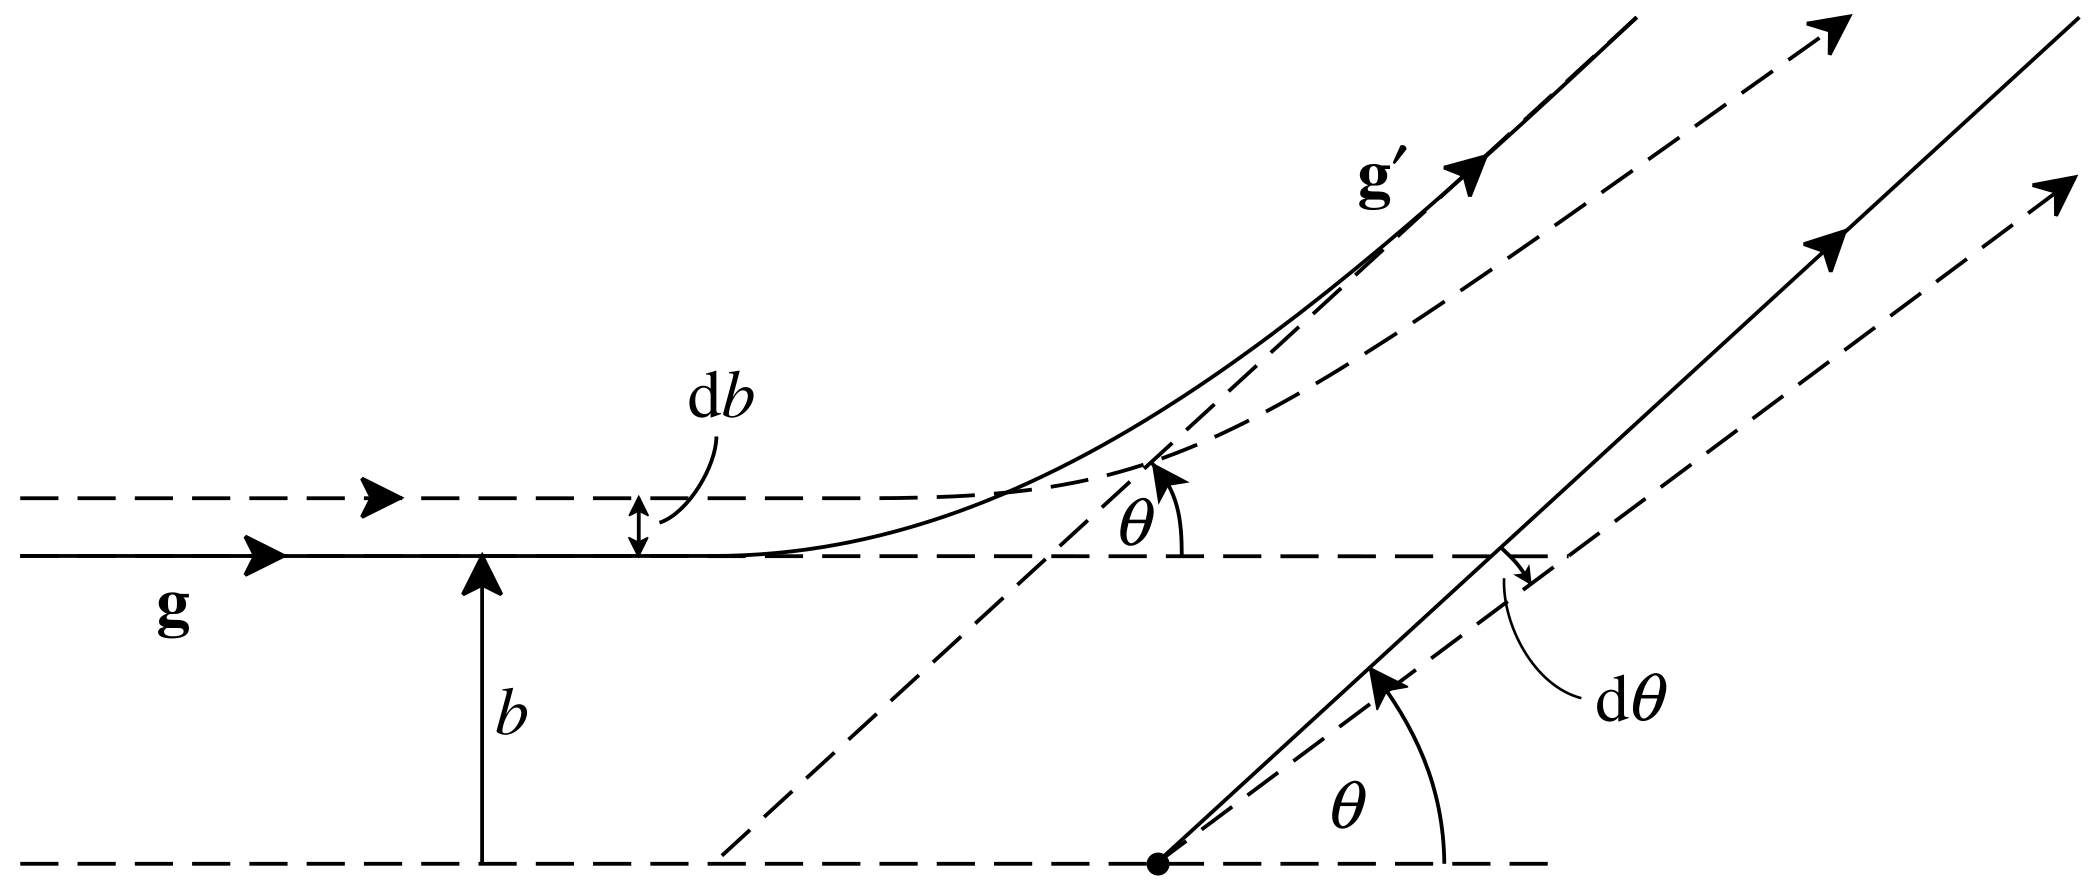
\includegraphics[width=0.63\textwidth]{figures/background/impact_parameter.png}
        \end{center}
        % \caption{Scattering in the center of mass frame (\cite{boyd_sanderson_2003}).}
        \label{fig:PICloopVel}
    \end{figure}

    \pause
    \begin{block}{Time Scale of Collisions}
        \begin{equation}
            \label{eq:timescales}
            \tau_c \ll \Delta t \ll \nu
        \end{equation}
    \end{block}

    \vspace{2mm}
    
    \item Collisions happen \textbf{locally} in configuration space (\cite{Callend2018Chapter3}) \\$\implies$ can assume collisions solely act on particle velocities

    \vspace{5mm}
    \begin{definitionBlock}
        \begin{tabular}{ll}
            $\tau_c$: & Collision Time \\
            $\nu$: & Dissipation Time
        \end{tabular}
    \end{definitionBlock}
\end{frame}

\begin{frame}{Fokker-Planck Equation}
    % \begin{itemize}
    %     \item FP operator = results from trunc. Taylor expansion
    %     \item FP describes time evolution of a velocity distribution under the influence of drag
    %     and random forces
    %     \item Bears similarity to Markov processes (i.e. brownian motion)
    %     \item And $\Delta \vect v \Delta \vect v$ is the change due to diffusion
    %     \item There exist many ways how to define the terms $\langle \Delta \vect v \rangle$ and
    %         $\langle \Delta \vect v \Delta \vect v \rangle$
    %     \item We'll take Rosenbluth's approach (formulate the potentials directly as poisson equations)
    %     \item Mention that we integrate over all possible scatterers of a certain velocity
    % \end{itemize}

    \onslide<1->
    \begin{block}{Fokker-Planck Equation}
        \begin{align}
            \label{eq:fokkerPlanckTerm}
            \left( \frac{\partial f}{\partial t} \right)_{\text{coll}} &= - \frac{\partial}{\partial \vect v}
            \cdot \left( f \frac{\langle \Delta \vect v \rangle }{\Delta t} \right) + \frac{1}{2}
            \frac{\partial^2}{\partial \vect v \partial \vect v} : \left( f \frac{ \langle \Delta \vect v
            \Delta \vect v \rangle}{\Delta t} \right)
        \end{align}
    \end{block}
    
    \vspace{3mm}

    \begin{columns}[onlytextwidth]
        \column{.47\textwidth}
        \onslide<2->{
            \begin{block}{Collision Coefficients\\\ }
                \begin{align}
                    \vect F_d(\vect v) = \frac{\langle \Delta \vect v \rangle}{\Delta t} &= \Gamma \frac{\partial h(\vect
                    v)}{\partial \vect v}, \label{eq:frictionCoeff} \eqVspace
                        \matr D(\vect v) = \frac{\langle \Delta \vect v \Delta \vect v \rangle}{\Delta t} &= \Gamma
                        \frac{\partial^2 g(\vect v)}{\partial \vect v \partial \vect v}. \label{eq:diffusionCoeff} 
                    \end{align}
                \end{block}
                \vspace*{\fill}
                \begin{definitionBlock}
                    \begin{tabular}{ll}
                        $\vect F_d(\vect v)$: & Dynamic friction coefficient \\
                        $\matr D(\vect v)$: & Stochastic diffusion coefficient
                    \end{tabular}
                \end{definitionBlock}
            }
            \onslide<3->{
                \column{.47\textwidth}
                \begin{block}{Poisson Problems \\ (\cite{rosenbluth}).}
                    \vspace{0.8mm}
                    \begin{align}
                        \velNabla^2 h(\vect v) &= -8 \pi f(\vect r, \vect v),
                        \label{eq:rbFirstPotential} \\[17pt]
                        \velNabla^2 \velNabla^2 g(\vect v) &= -8 \pi f(\vect r, \vect v). \label{eq:rbSecondPotential}
                    \end{align}
                \end{block}
            }
        \end{columns}


\end{frame}

\section{Methods}

\begin{frame}{Particle-in-Cell Overview}
    % \begin{itemize}
    %     \item We introduced the theory, but how do we transfer this into a numerical code?
    %     \item Use widely applied PIC methods (electrostatic PIC + velocity PIC)
    %     \item Talk about why we use those boundary conditions...
    % \end{itemize}

    \begin{center}
    % Configuration space PIC loop
    \begin{overprint}
        \onslide<1>
        \begin{center}
        \item Electrostatic PIC with \textbf{Periodic} boundary conditions.
        \end{center}
        \begin{figure}
            \begin{center}
                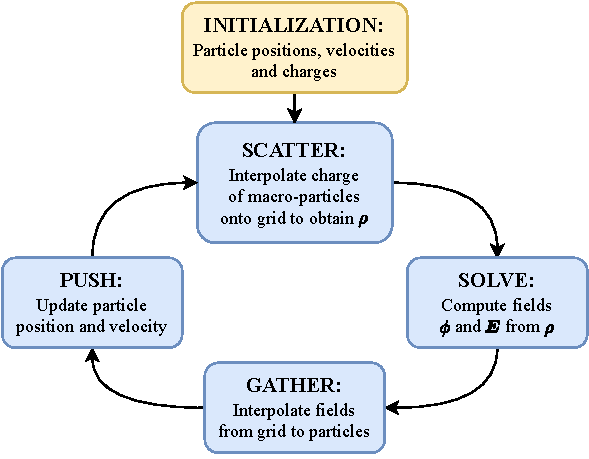
\includegraphics[width=0.7\textwidth]{figures/computational_model/PICloop_electrostatic.pdf}
            \end{center}
            % \caption{Electrostatic PIC with \textbf{Periodic} boundary conditions.}
            \label{fig:PICloopConfig}
        \end{figure}

        % Velocity space PIC loop
        \onslide<2>
        \begin{center}
        \item Velocity PIC with \textbf{Open} boundary conditions.
        \end{center}
        \begin{figure}
            \begin{center}
                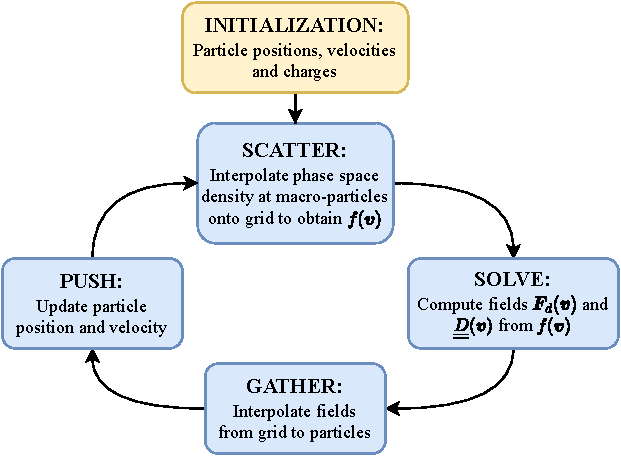
\includegraphics[width=0.74\textwidth]{figures/computational_model/PICloop_velocity.pdf}
            \end{center}
            % \caption{Velocity PIC with \textbf{Open} boundary conditions.}
            \label{fig:PICloopVel}
        \end{figure}
    \end{overprint}

    \end{center}
\end{frame}

        
\begin{frame}{Resulting Scheme}

    % \begin{itemize}
    %     \item We've talked about the randomness in how these collisions happen, how do we reflect
    %     this in the timestepping procedure?
    %     \item Langevin Eq. arises naturaly when a variable experience a slow time variation in
    %         velocity due to many small random forces.
    %     \item Akin to the idea of Markov processes. Where the current state only depends on the
    %         previous one and thus has no memory.
    %     \item Metion why we chose LDLT decomposition (Matrices should at least be s.p.d.)
    % \end{itemize}

    \onslide<1->
    \begin{block}{FP Equation $\Longleftrightarrow$ Langevin Equation
        (\cite{tabar2019})}
    \begin{align}
        d\vect v(t) &= \underbrace{\vect a(\vect v, t)}_{\vect F_d(\vect v)} dt + \underbrace{\vect
        b(\vect v, t)}_{\matr Q(\vect v)} d\vect W (t), \eqVspace
            d\vect W(t) &= \vect \xi_t dt, \quad \vect \xi_t \sim \mathcal N(0,1).
    \end{align}
    \end{block}

    \onslide<2->
    \begin{exampleblock}{LDLT factorization for positive semi-definite Matrices}
        \begin{equation}
            \matr D = \matr L \matr S^2 \matr L^T \implies \matr Q = \matr S \matr L^T, 
        \end{equation}
        \item where $\matr D$ is positive semi-definite (\cite{hinton1983collisional}).
    \end{exampleblock}


    \onslide<1->

    % \vspace*{\fill}
    \vspace{2cm}
    \begin{definitionBlock}
         \begin{tabular}{ll}
             $\vect F_d(\vect v)$: & Dynamic friction coefficient \\
             $\matr D(\vect v)$: & Stochastic diffusion coefficient
        \end{tabular}
    \end{definitionBlock}

\end{frame}

\begin{frame}[c]{Resulting Scheme}

    % Remove spacing before and after algorithm environment
    \setlength{\intextsep}{0pt}
    \begin{exampleblock}{}
        \begin{algorithm}[H]
            \caption{Euler-Maruyama Time Integrator Procedure.}
            \label{alg:integrator}
            \begin{algorithmic}[1]
                \addtocounter{algorithm}{-1} % Adjust the algorithm counter (otherwise it increases in every slide)
                \Procedure{Advance Particles in time by $dt$}{}
                \visible<1->{\State $\vect r \gets \vect r + \frac{dt}{2} \vect v$;}
                \visible<1->{\State Compute $\vect F(\vect r)$; $\vect v \gets \vect v +
                    \frac{dt}{2} \frac{\vect F}{m}$;
                \hfill\COMMENT{\textcolor{gray!120}{(Electrostatic PIC)}}}
                \visible<2->{\State Compute $\vect F_d(\vect v)$ and $\matr D(\vect v)$;
                \hfill\COMMENT{\textcolor{gray!120}{(Velocity PIC)}}}
                \visible<3->{\State Factorize $\matr D(\vect v)$; $\matr Q \gets \matr S \matr L^T$;
                \hfill\COMMENT{\textcolor{gray!120}{(LDLT Factorization)}}}
                \visible<4->{\State $\vect v \gets \vect v + dt \vect F_d + d\vect W(t) \cdot \matr Q$;}
                \visible<5->{\State Compute $\vect F(\vect r)$; $\vect v \gets \vect v +
                    \frac{dt}{2} \frac{\vect
                F}{m}$;\hfill\COMMENT{\textcolor{gray!120}{(Electrostatic PIC)}}}
                \visible<5->{\State $\vect r \gets \vect r + \frac{dt}{2} \vect v$;
                \EndProcedure.}
            \end{algorithmic}
        \end{algorithm}
    \end{exampleblock}
\end{frame}

% Enable caption numbering again
\setbeamertemplate{caption}[numbered]

\section{Results}

\begin{frame}{Convergence Study: Rosenbluth Potentials}
    % \begin{itemize}
    %     \item Why is it important to have an analytical test case? We were able to test for
    %         $h(\vect v)$, $g(\vect v)$, $\nabla h(\vect v)$, $\matr D(\vect v)$
    %     \item State initial phase space distribution $f(\vect v)$
    %     \item Say that we've tested FD and spectral (here we show spectral). Both show 2nd order
    %     convergence
    %     \item We need to scale Domain for velocity PIC with Hockney's method (no need to
    %         write down)
    %     \item Mention that we've tested the cholesky decomposition (no need to write down)
    %     \item We also found overall many interesting behaviors which we couldn't entirely explain
    %     (e.g. the spectral method showing worse convergence than FD)
    % \end{itemize}

    \begin{block}{Gaussian Initial Velocity Density}
        \begin{equation}
            f(\vect v) = \frac{1}{\sqrt{8 \pi^3} \sigma^3}
            \exp{\left( -\frac{v^2}{2 \sigma^2} \right)}, \quad \sigma = 0.05 v_{max}
            \label{eq:gaussianDensity}
        \end{equation}
    \end{block}
    
    \only<1->
    \begin{block}{Relative approximation error $\eta$}
        \begin{equation}
            \eta(x, x_{\text{appr}}) = \frac{\lVert x_{\text{appr}}-x \rVert_2}{\lVert x \rVert_2}
        \end{equation}
    \end{block}

    % \vfill
    % \begin{definitionBlock}
    %      \begin{tabular}{ll}
    %          $\eta(x, x_{\text{appr}}):$ & Relative approximation error
    %     \end{tabular}
    % \end{definitionBlock}

\end{frame}

\begin{frame}{Convergence Study: Rosenbluth Potentials}
    % \begin{itemize}
    %     \item As mentioned we have many possible solver combinations at our disposal in our limited
    %         survey we came to the conclusion that the following is a good candidate
    %     \item Poisson solvers Vico/Hockney
    %     \item FD or spectral gradient/Hessian
    % \end{itemize}

    \begin{block}{Gaussian Initial Velocity Density}
        \begin{equation}
            f(\vect v) = \frac{1}{\sqrt{8 \pi^3} \sigma^3}
            \exp{\left( -\frac{v^2}{2 \sigma^2} \right)}, \quad \sigma = 0.05 v_{max}
            \label{eq:gaussianDensity}
        \end{equation}
    \end{block}
    
    \only<0->{
    \begin{columns}[1.1\textwidth]
        \column{.5\textwidth}
        \onslide<1->{
            \begin{figure}
                \begin{center}
                    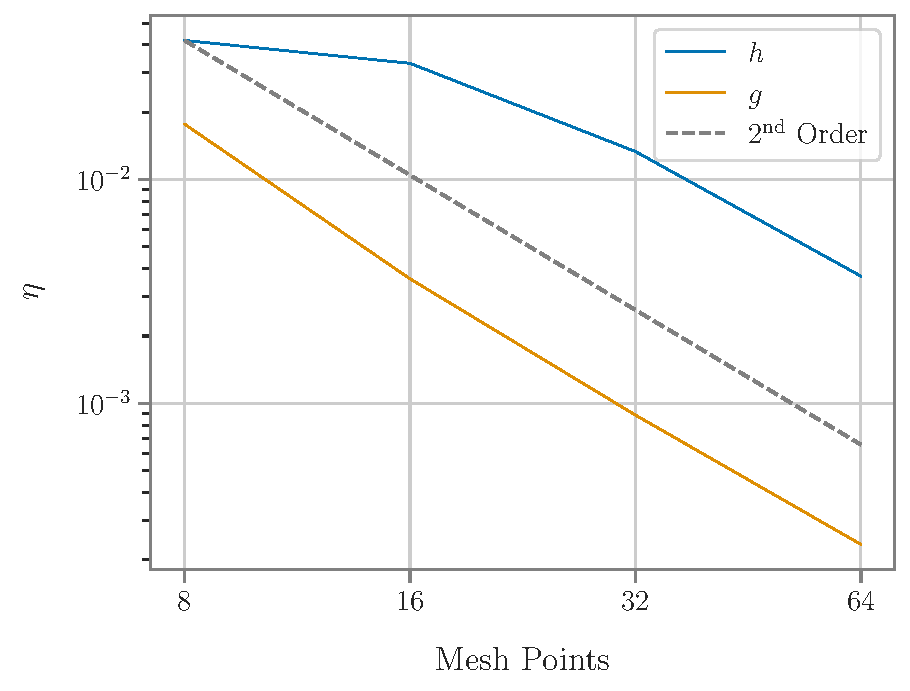
\includegraphics[width=\textwidth]{figures/results/convergenceStudy/hg_005vmax_VICO.pdf}
                \end{center}
                % \caption{Electrostatic PIC with \textbf{Periodic} boundary conditions.}
                \label{fig:convergence_DFd_VICO_FD}
            \end{figure}
        }
        \onslide<2->{
            \column{.5\textwidth}
            \begin{figure}
                \begin{center}
                    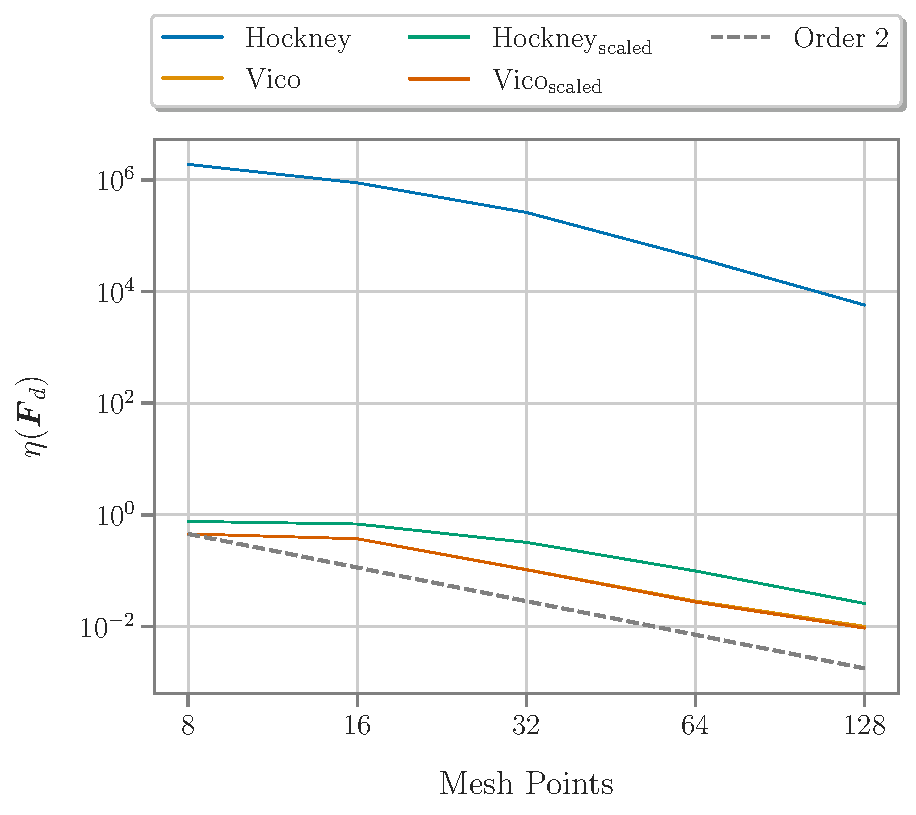
\includegraphics[width=\textwidth]{figures/results/convergenceStudy/Fd_joint_comparison.pdf}
                \end{center}
                % \caption{Electrostatic PIC with \textbf{Periodic} boundary conditions.}
                \label{fig:convergence_DFd_VICO_spectral}
            \end{figure}
        }
    \end{columns}
}

\end{frame}

\begin{frame}{Disorder Induced Heating (DIH) Test Case}
    % \begin{itemize}
    %     \item Need system where collisions play major part in dynamics -> relaxation to thermal
    %         equilibrium
    %     \item Happens in ultracold plasmas with low kinetic energy
    %     \item Initially unstructured particles start to interact (coulomb)
    %     \item heat up the system by transfering pot. E to kin. E. -> heating up the system
    % \end{itemize}

    \only<2->{
        \begin{block}{\pcubem Reference Implementation}
            \begin{itemize}
                \itemVspace
                \item \pcubem $\equiv$ (Particle-Particle Particle-Mesh) by \cite{Hockney2021}, \cite{p3m_ulmer}
                \item High computational complexity 
                \item 2 hyperparameters (cut-off radius $r_c$, interaction splitting parameter $\alpha$)
            \end{itemize}
        \end{block}
    }

    \only<3->{
        \begin{block}{Cold Sphere Initial Condition (\cite{mitchell2015parallel})}
            \begin{itemize}
                \itemVspace
                \item $N_p = 156055$ electrons in a sphere of radius $R = 17.74\ \mu m$ $\implies \tau_p = 4.31 \times 10^{-11}\ s$
            \item Simulation time: $t_{tot} = 5\tau_p$, $dt=2.15623\times 10^{-13}\ s \implies 1000\ dt$
                \item Particles initially at rest: $\vect v(t = 0) = 0$
                \item Normalized x-emittance at equilibrium: $\neps = 0.491\ nm$
                    % \item Plasma period $\tau_p = 4.31 \times 10^{-11}\ s$
            \end{itemize}
        \end{block}
    }

    \vspace{0.8cm}

    \only<3->{
        \begin{definitionBlock}
            \begin{tabular}{ll}
                $\tau_p$: & Plasma period \\
                $\neps$: & Normalized x-emittance
            \end{tabular}
        \end{definitionBlock}
    }
\end{frame}

\begin{frame}{Disorder Induced Heating (DIH) Test Case}
    % \begin{itemize}
    %     \item As mentioned we have many possible solver combinations at our disposal in our limited
    %         survey we came to the conclusion that the following is a good candidate
    % \end{itemize}

    \begin{center}
        \item Solver setup for the DIH experiments:
            \begin{table}
                \renewcommand*\arraystretch{1.5}
                \centering
                \label{table:DIHsolverCombination}
                \begin{tabular}{|l|l|l|}
                    \hline
                    \textbf{PIC Type}                           & \textbf{Quantity of Interest}
                                                                & \textbf{Comp. Domain or Method}     \\ \hline
                    {Electrostatic PIC} &  $- \posNabla \left[ \phi(\vect r) \right]$ & Spectral Gradient: $\spPosNabla$          \\ \hline
                    \multirow{2}{*}{Velocity PIC}      & $\velNabla h(\vect v)$, $g(\vect v)$                                        
                                                       & \cite{vicoGreengard2016} + $\spVelNabla$                       \\ \cline{2-3} 
                                                       & $\frac{\partial^2}{\partial \vect v \partial \vect v} g(\vect v)$
                                                       & FD Hessian: $\fdVelHess$           \\
                                                       \hline
                \end{tabular}
            \end{table}
        \vfill
            \begin{definitionBlock}
                \begin{tabular}{ll}
                    $\star^{\text{fd}}:$ & Operator computed with Finite Difference (FD) \\
                    $\star^{\text{sp}}:$ & Operator computed with a spectral method (\cite{vicoGreengard2016})
                \end{tabular}
            \end{definitionBlock}
        \end{center}
\end{frame}


\begin{frame}[c]{DIH Baseline (no collision)}
    % \begin{itemize}
    %     \item Collisionless baseline case: We couldn't explain why the spectral gradient results in 
    %     \item The trend doesn't stop for long times
    %     \item Periodic behavior more regular with our method
    % \end{itemize}

    \centering
    \item Normalized x-emittance $\neps$ of collisionless Langevin solver and \pcubem.
    \begin{figure}
        \begin{center}
            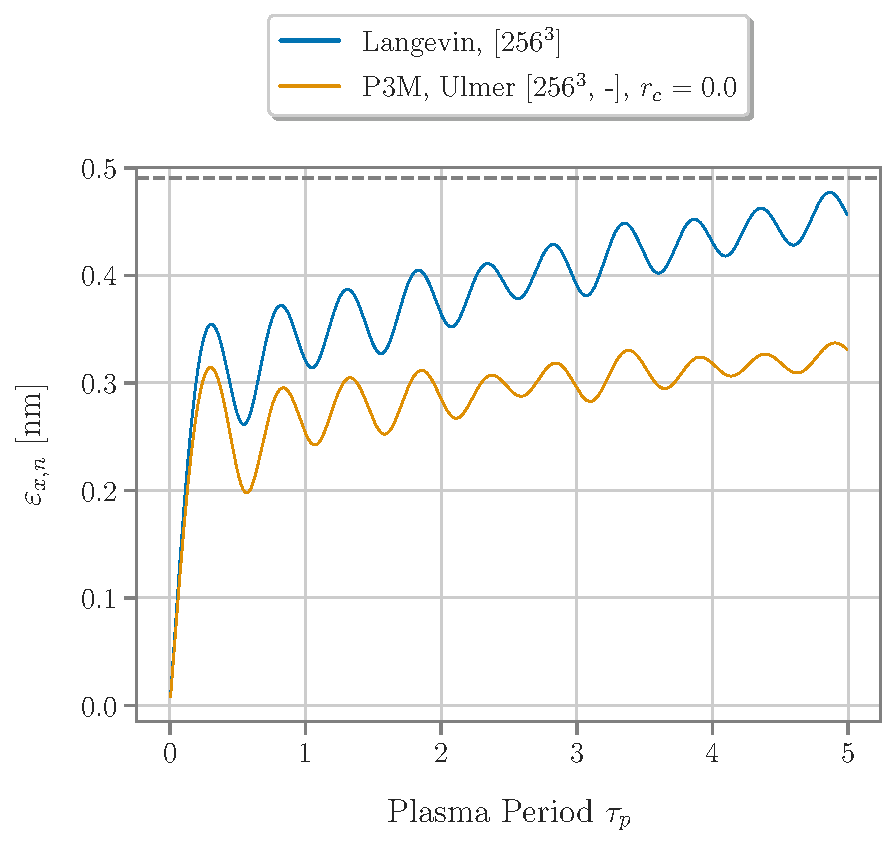
\includegraphics[width=0.55\textwidth]{figures/presentation_only/langevin_baseline.pdf}
        \end{center}
        % \caption{Normalized x-emittance $\neps$ of collisionless Langevin solver and \pcubem.}
        \label{fig:gamma_test}
    \end{figure}
\end{frame}

\begin{frame}{Friction \& Diffusion Coefficient}
    % \begin{itemize}
    %     \item Average norm of friction over time
    %     \item Starts off with zero friction (due to zero vel. distr.)
    %     \item Will reach a limit similar to the emittance
    %     \item Magnitude times dt is not large enough to impact eps
    %
    %     \item Attention: Log scale -> different magnitudes (sheer stresses due to collisions much
    %     smaller)
    %     \item Sheer stresses much more sensitive to the initial condition / need longer warmup
    %     time
    % \end{itemize}

    \begin{itemize}
        \itemVspace
        \item<2-> Friction coefficients on their own are not large enough to impact $\neps$.
        \item<3-> Diagonal diffusion coefficients are indeed dominant (\cite{manheimer1997langevin}).
            \vspace{0.75cm}
    \end{itemize}

    \begin{columns}[1.1\textwidth]
        \column{.5\textwidth}
        \onslide<1->{
            \vspace{0.50cm}
            \begin{figure}
                \begin{center}
                    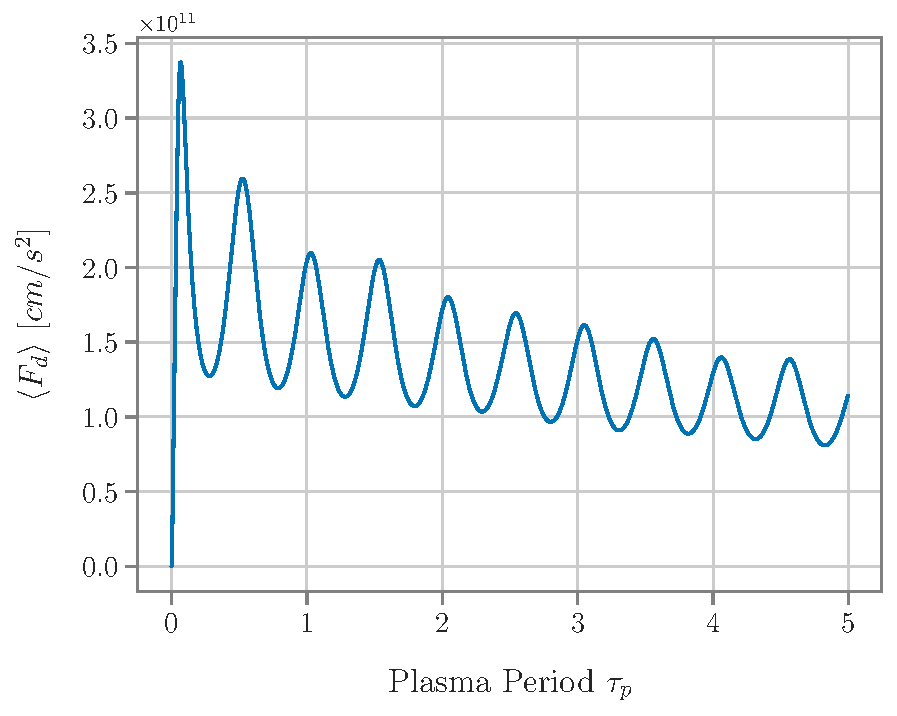
\includegraphics[width=1.0\textwidth, keepaspectratio, valign=b]{figures/results/Fd_avg.pdf}
                \end{center}
                % \caption{Electrostatic PIC with \textbf{Periodic} boundary conditions.}
                \label{fig:convergence_DFd_VICO_FD}
            \end{figure}
        }
        \onslide<3->{
            \column{.5\textwidth}
            \begin{figure}
                \begin{center}
                    \begin{tikzpicture}
                        \node[anchor=south west,inner sep=0] at (0,0) {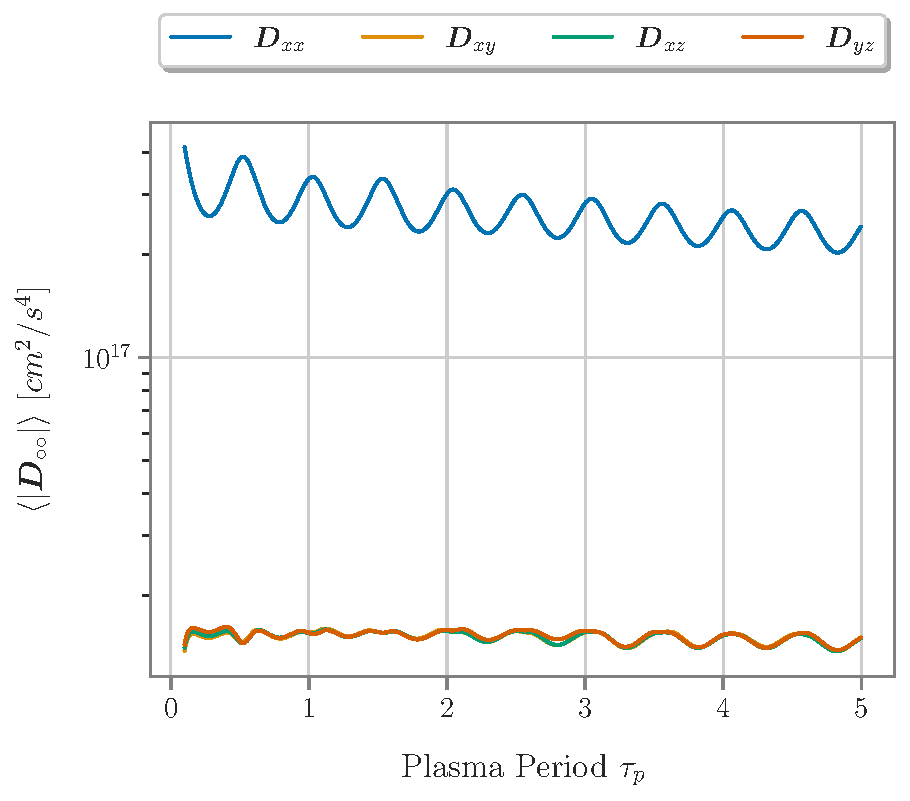
\includegraphics[width=\textwidth, keepaspectratio, valign=b]{figures/results/D_avg.pdf}};
                    \end{tikzpicture}
                \end{center}
                % \caption{Electrostatic PIC with \textbf{Periodic} boundary conditions.}
                \label{fig:convergence_DFd_VICO_spectral}
            \end{figure}
        }
    \end{columns}
\end{frame}

\begin{frame}{Friction \& Diffusion Coefficient}
    \begin{itemize}
        \itemVspace
        \item Friction coefficients are too small to impact $\neps$.
        \item Diagonal diffusion coefficients are indeed dominant (\cite{manheimer1997langevin}).
        \item Off-diagonal values show non-periodic behavior for $t < 3\tau_p$.
    \end{itemize}

    \begin{columns}[1.1\textwidth]
        \column{.5\textwidth}
            \vspace{0.50cm}
            \begin{figure}
                \begin{center}
                    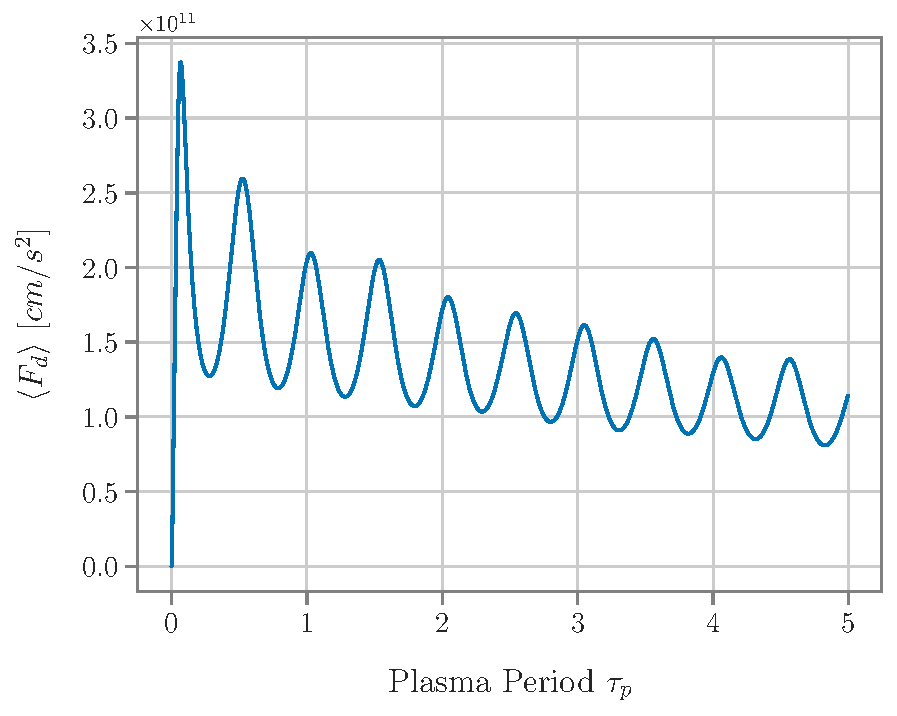
\includegraphics[width=1.0\textwidth, keepaspectratio, valign=b]{figures/results/Fd_avg.pdf}
                \end{center}
                % \caption{Electrostatic PIC with \textbf{Periodic} boundary conditions.}
                \label{fig:convergence_DFd_VICO_FD}
            \end{figure}
            \column{.5\textwidth}
            \begin{figure}
                \begin{center}
                    \begin{tikzpicture}
                        \node[anchor=south west,inner sep=0] at (0,0) {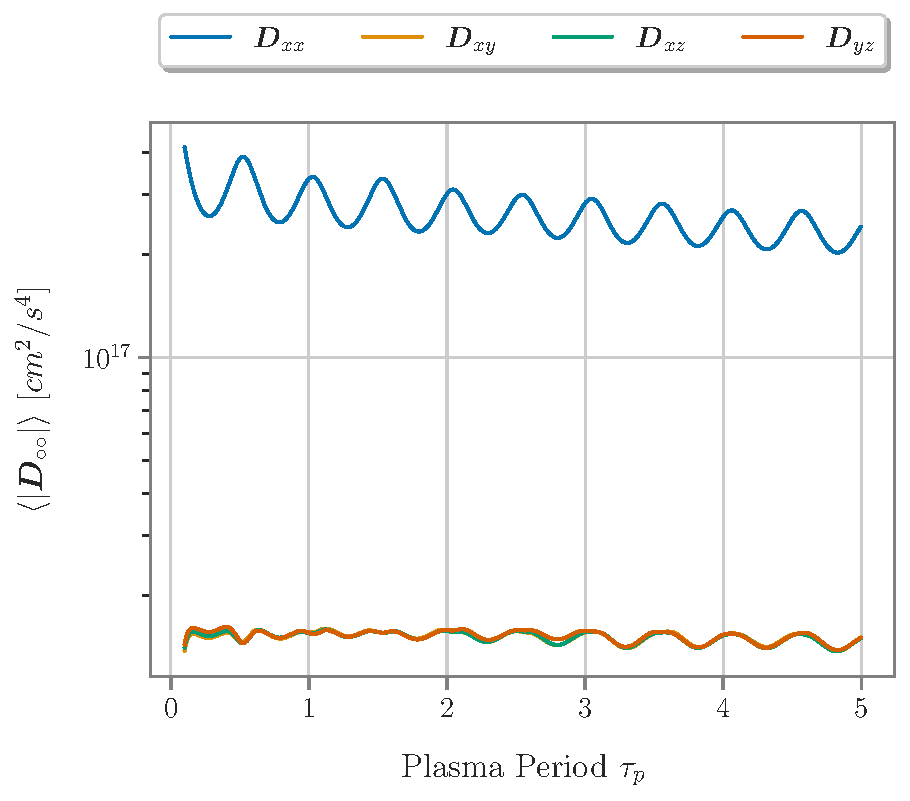
\includegraphics[width=\textwidth, keepaspectratio, valign=b]{figures/results/D_avg.pdf}};
                        \draw<1>[red,thick,rounded corners] (1.0,1.25) rectangle (3.5,0.75);
                    \end{tikzpicture}
                \end{center}
                % \caption{Electrostatic PIC with \textbf{Periodic} boundary conditions.}
                \label{fig:convergence_DFd_VICO_spectral}
            \end{figure}
    \end{columns}

\end{frame}

\begin{frame}{Investigation of Diffusion Coefficients $\matr D$}
    \begin{itemize}
        \itemVspace
        \item<1-> Diffusion matrices not only positive semi-definite (inhibits LDLT decomposition)
        \item<3-> Negative definite matrices start to vanish after $t = 3\tau_p$
    \end{itemize}
    
    \only<2->{
        \begin{figure}
            \begin{center}
                \hspace*{-1.0cm}
                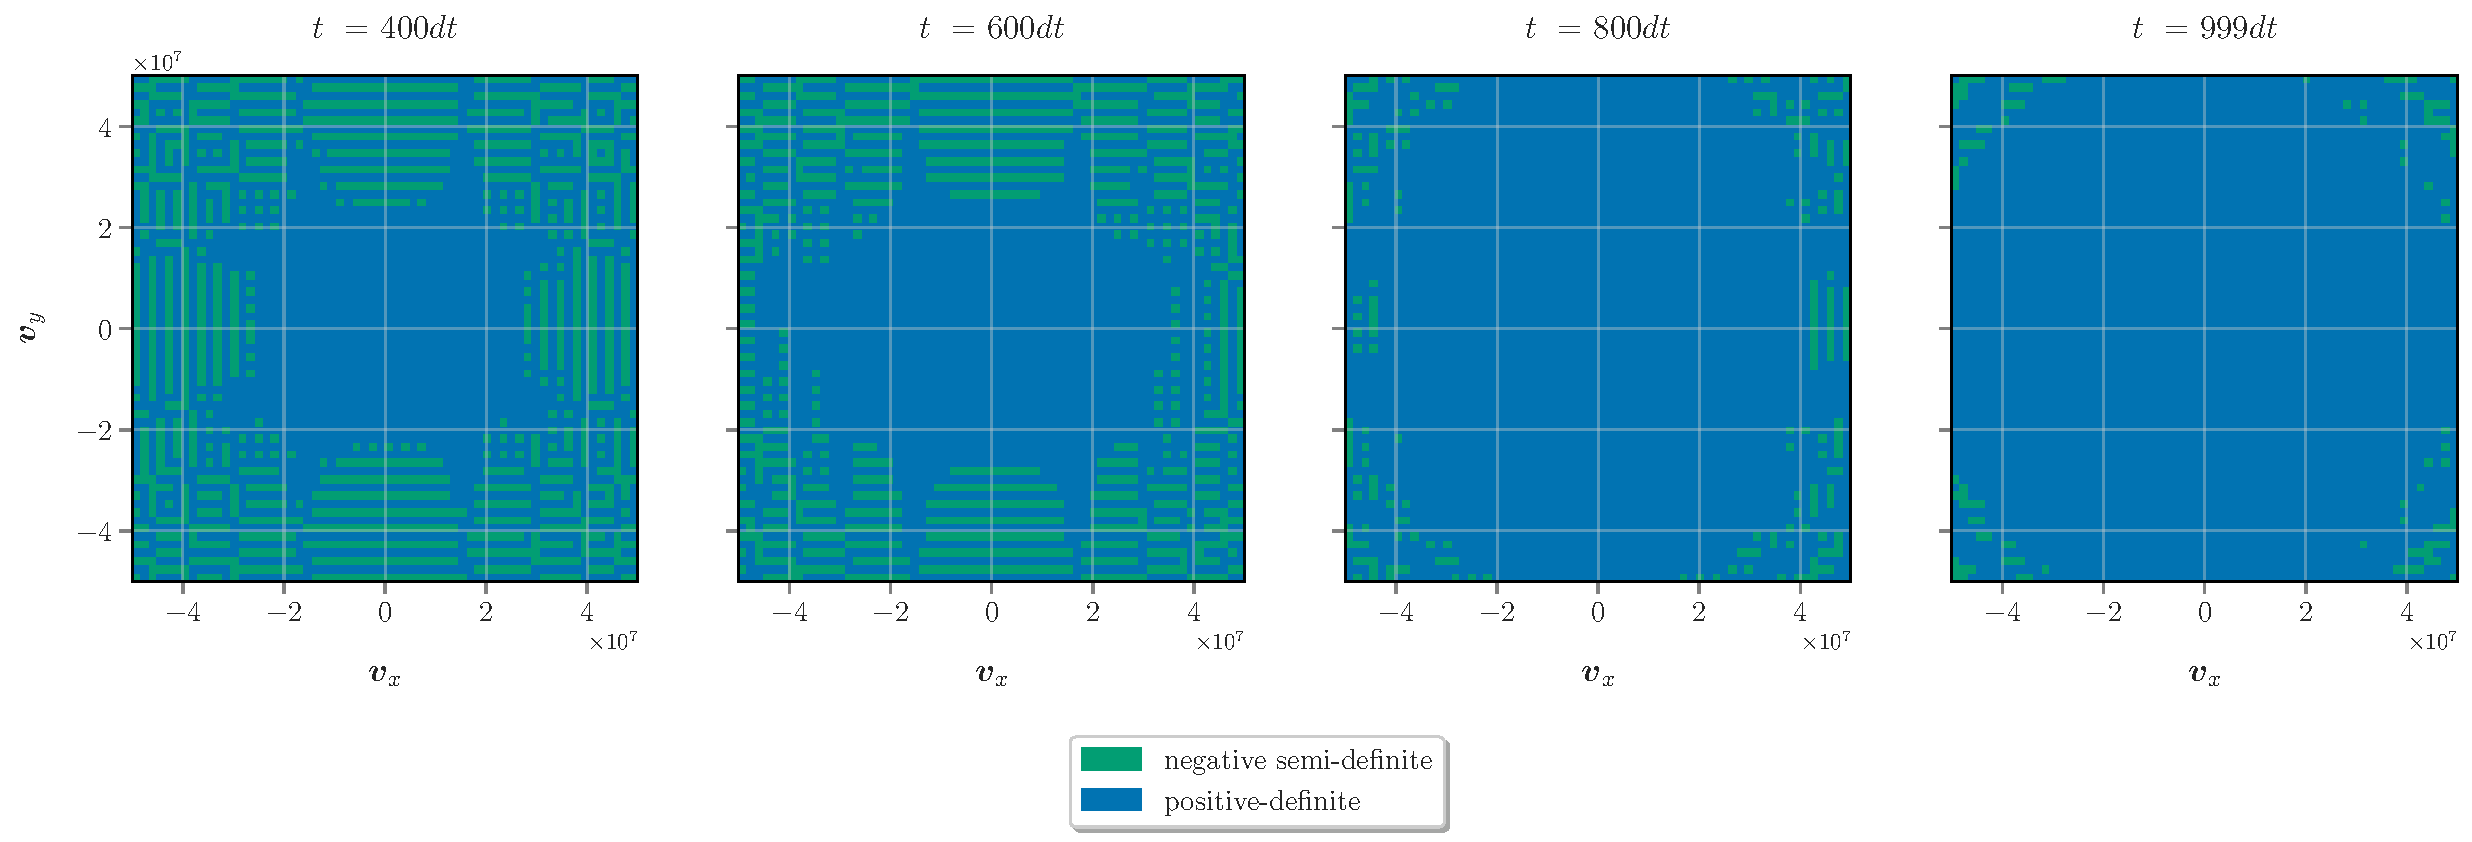
\includegraphics[width=1.15\textwidth]{figures/results/D_cholesky_time.pdf}
            \end{center}
            % \caption{Evolution of a slice through the diffusion matrix field at $\vect v_z = 0$ over time.}
            \label{fig:D_cholesky_time}
        \end{figure}
    }
\end{frame}

\section{Summary}

\begin{frame}[c]{Conclusion}

    \begin{block}{Langevin Solver for the Vlasov-Poisson-Vokker-Planck equation}
    \begin{itemize}
        \itemVspace
        \setlength\itemsep{1.5em}
        \item<1-> Better complexity than reference solver (\pcubem) / less hyperparameters
        \item<2-> Verified correctness of collision operator on analytical test cases
        \item<3-> Investigated impact of two solver types on normalized emittance
        \item<4-> Friction coefficient exhibits no impact on DIH test case
        \item<5-> Negative definite diffusion matrices inhibit adding diffusive term in time integration
    \end{itemize}
    \end{block}
\end{frame}

\begin{frame}[c]{Conclusion}

    \begin{block}{\large Outlook}
        \begin{itemize}
            \itemVspace
            \setlength\itemsep{1.5em}
            \item<1-> Investigate noise in diffusion matrices for $t < 3\tau_p$ %(Eigenvalue analysis / check
                %how only taking diagonal values impacts decomposition)
            \item<2-> Investigate $dt / h_v$ interplay in the symmetric time integrator (i.e. subcycling)
            \item<3-> Test convserving time integrator (high order SDE methods)
            \item<4-> Test on a simpler physical test case
            \item<5-> Performance improvements:
                \begin{itemize}
                    \item<5-> Asynchronous computation of $\vect F_d(\vect v)$ and $\matr D(\vect v)$
                    \item<5-> MPI parallelization via ``Super-Cell'' approach (\cite{qiang2000self})
                \end{itemize}
        \end{itemize}
    \end{block}

    \vspace*{\fill}
    \begin{definitionBlock}
         \begin{tabular}{ll}
             $h_v$: & Mesh width in velocity space\\
        \end{tabular}
    \end{definitionBlock}
\end{frame}

% \subsection{Thank you!}

\appendix
\section{Appendix}

\begin{frame}{Appendix I: Explored Solver components}
\item Possible ways of defining the electrostatic Poisson problem:
    \begin{figure}
        \begin{center}
            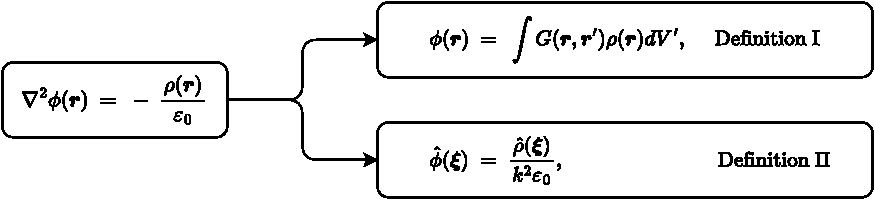
\includegraphics[width=0.88\textwidth]{figures/results/greenPoisson.pdf}
        \end{center}
        % \caption{Two mathematically identical formulations of the solution to the Poisson problem
        % \ref{eq:poissonEquation}. As used in Table \ref{table:langevinPossibleMethods}.}
        \label{fig:greenPoissonDefinitions}
    \end{figure}

    \begin{table}[h]
        \renewcommand*\arraystretch{1.5}
        \centering
        % \caption{Overview of explored  methods for the various quantities needed by the Langevin solver.}
        \label{table:langevinPossibleMethods}
        \begin{tabular}{|l|l|l|}
            \hline
            \textbf{PIC Type}                           & \textbf{Quantity of Interest}
                                                              & \textbf{Comp. Domain or Method}     \\ \hline
            \multirow{4}{*}{Electrostatic PIC} & \multirow{2}{*}{$\phi(\vect r)$}
                                                     & Definition I (see Fig. above)  \\ \cline{3-3} 
                                                     &
                                                     & Definition II (see Fig. above)  \\ \cline{2-3} 
                                                     & \multirow{2}{*}{$- \posNabla \phi(\vect r)$}
                                                     & Finite Difference Gradient: $\fdPosNabla$ \\ \cline{3-3} 
                                                     &
                                                     & Spectral Gradient: $\spPosNabla$          \\ \hline
            \multirow{4}{*}{Velocity PIC}      & \multirow{2}{*}{$\velNabla h(\vect v)$, $g(\vect v)$}
                                                     & Hockney, $ \velNabla^{\{\text{fd,sp}\}} $                      \\ \cline{3-3} 
                                                     &
                                                     & Vico, $ \velNabla^{\{\text{fd,sp}\}} $                      \\ \cline{2-3} 
                                                     & \multirow{2}{*}{$\frac{\partial^2}{\partial \vect v \partial
    \vect v} g(\vect v)$} & Finite Difference Hessian: $\fdVelHess$ \\ \cline{3-3} 
                          &
                          & Spectral Hessian: $\spVelHess$           \\
                          \hline
\end{tabular}
\end{table}
\end{frame}

\begin{frame}{Appendix II: Varying Poisson Solver Type}
    \begin{figure}
        \begin{center}
            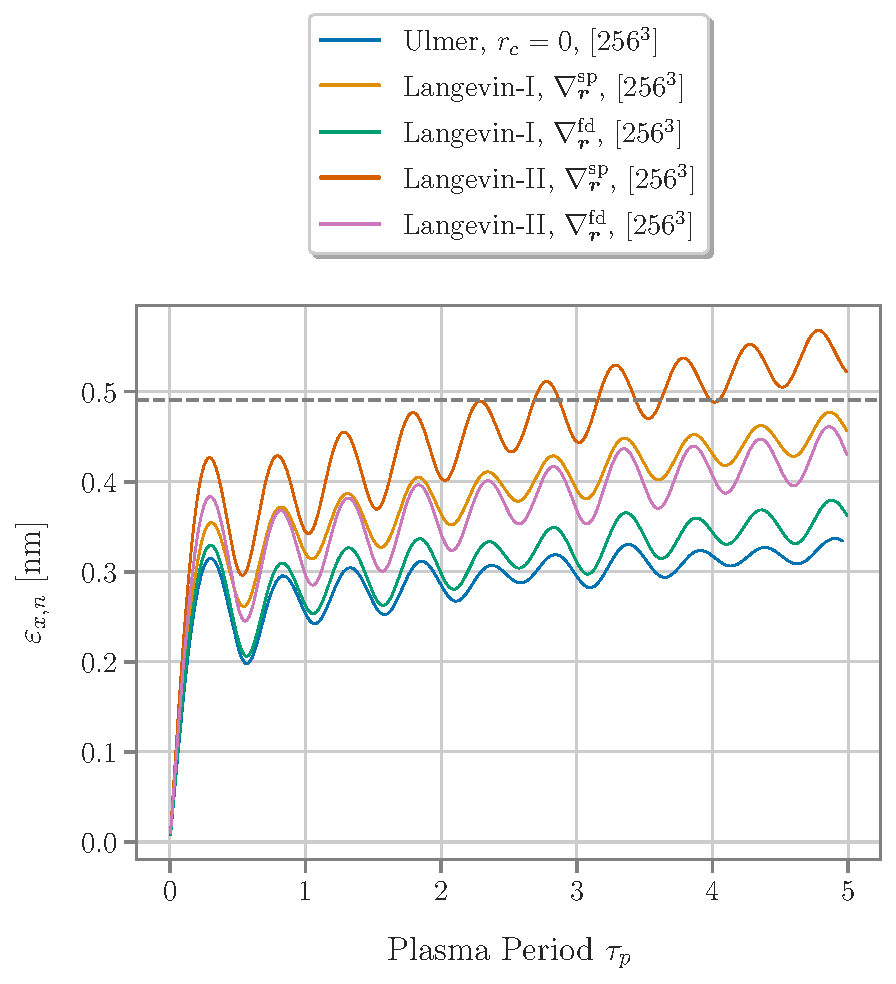
\includegraphics[width=0.62\textwidth]{figures/results/Efield_gradient_test.pdf}
        \end{center}
            % \caption{Varying solver type.}
            \label{fig:EfieldGradientTest}
    \end{figure}
\end{frame}

\begin{frame}{Appendix III: Varying Poisson Solver Mesh Size}
    \begin{figure}
        \begin{center}
            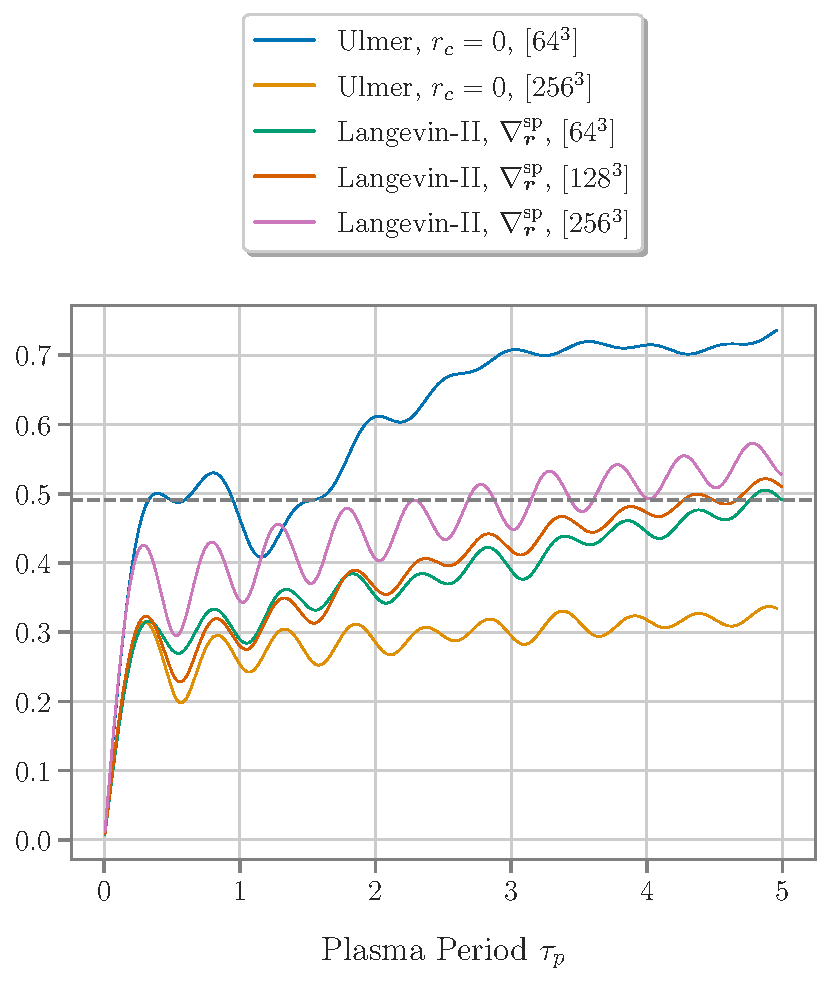
\includegraphics[width=0.58\textwidth]{figures/results/meshsize_test.pdf}
        \end{center}
            % \caption{Varying mesh size.}
            \label{fig:meshsize_test_VICO}
    \end{figure}
\end{frame}

\begin{frame}{Appendix IV: Convergence of Coefficients}
\item Convergence study of collisional coefficients for a Gaussian
        velocity distribution which models the distribution of the \gls{dih} problem.
    \begin{figure}[h]
        \begin{subfigure}[b]{0.5\textwidth}
            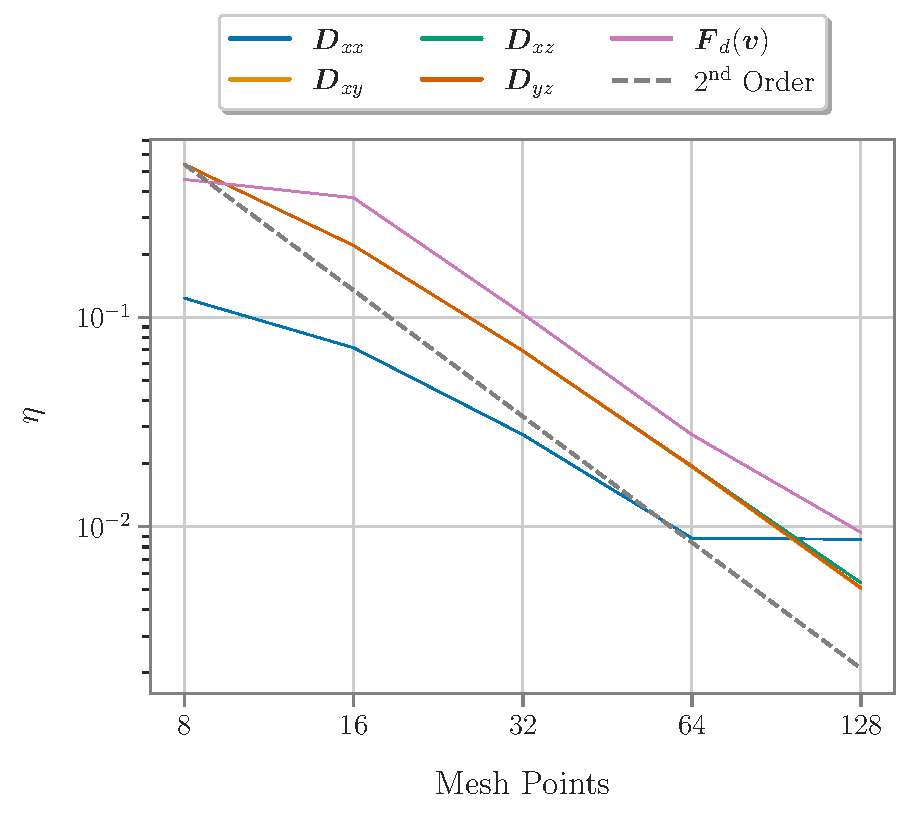
\includegraphics[width=\textwidth]{figures/results/convergenceStudy/D+Fd_005vmax_VICO.pdf}
            \caption{Finite Difference computation of coefficients.}
            \label{fig:convergence_DFd_VICO_FD}
        \end{subfigure}
        \hfill
        \begin{subfigure}[b]{0.465\textwidth}
            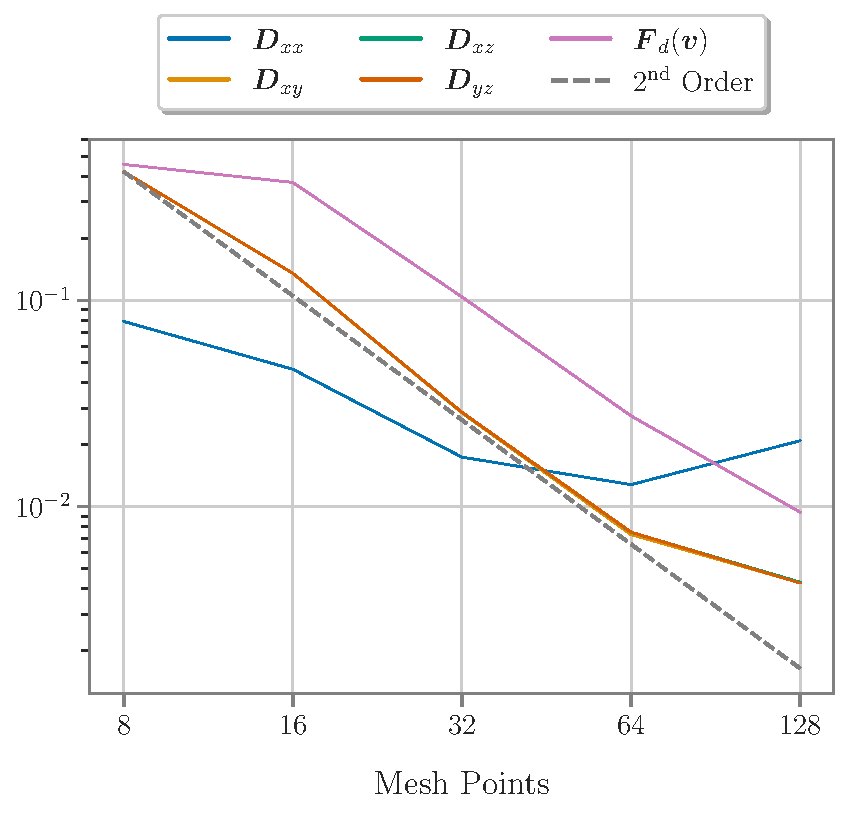
\includegraphics[width=\textwidth]{figures/results/convergenceStudy/D+Fd_005vmax_VICO_spectralHess.pdf}
            \caption{Spectral computation of coefficients.}
            \label{fig:convergence_DFd_VICO_spectral}
        \end{subfigure}
        % \caption{Convergence study of collisional coefficients for a Gaussian
        % velocity distribution which models the distribution of the \gls{dih} problem.}
        \label{fig:convergence_VICO_spectral_FD_comparison}
    \end{figure}
\end{frame}

\begin{frame}{Appendix V: Friction \& Diffusion Coefficients}
    Friction coefficient does not have any impact on DIH $\neps$:
    \begin{figure}[h]
        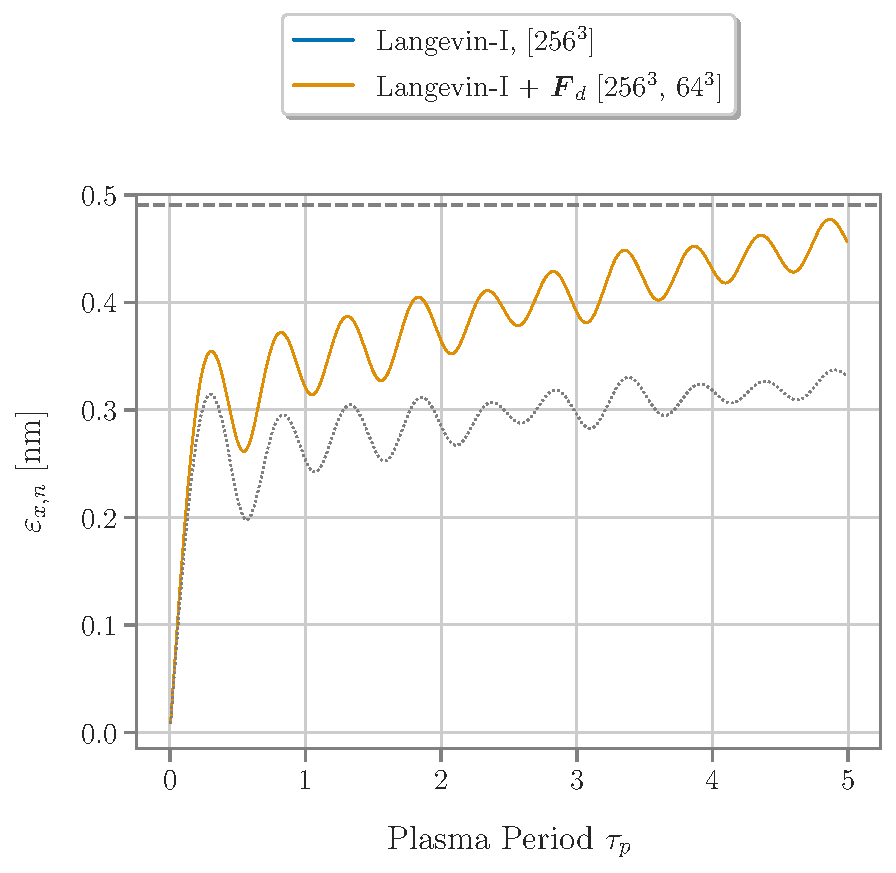
\includegraphics[width=0.6\textwidth, keepaspectratio, valign=b]{figures/results/Langevin_Fd.pdf}
        % \caption{Langevin Solver on the DIH test case with and without friction enabled.}
        \label{fig:Fd_DIH}
    \end{figure}
\end{frame}

\begin{frame}[fragile]{Appendix VI: Chainable differential operators}
    \lstinputlisting[caption={Pseudo-code for a chained operator (equivalent to
    $\frac{\partial^2}{\partial x \partial y} f(x,y)$).}, label={lst:stencils}, language=C++]{./code_snippets/diffOperator/chainableOperator.cpp}
\end{frame}

\begin{frame}{Appendix VII: Chainable differential operators}
    \begin{figure}
        \begin{center}
            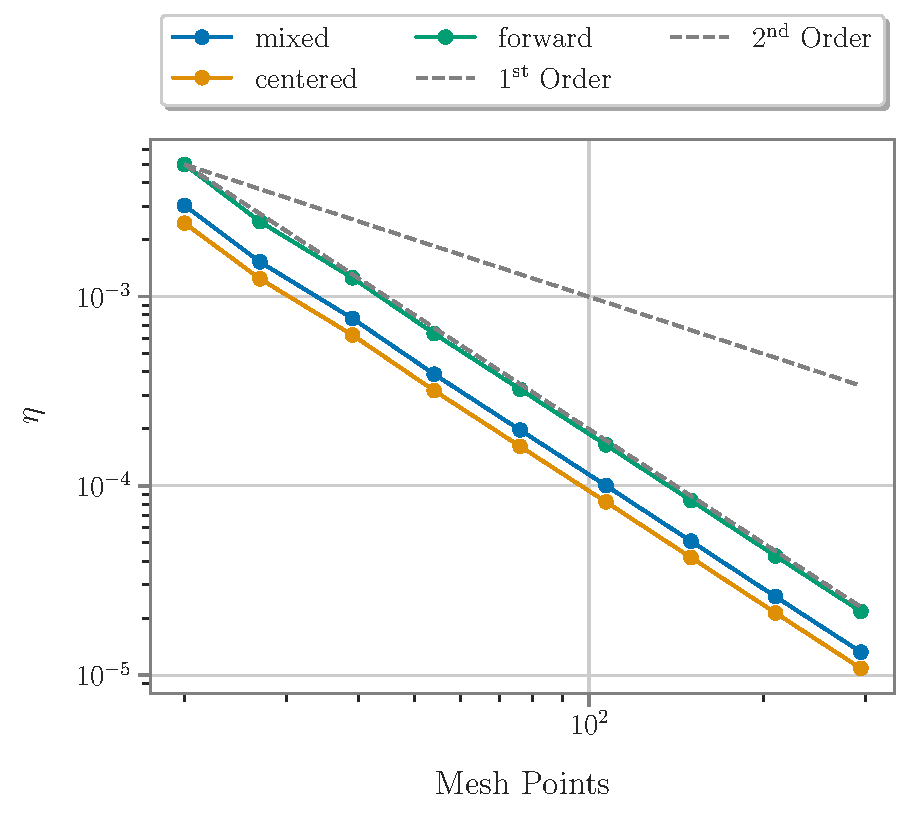
\includegraphics[width=0.62\textwidth]{figures/appendix/chainableOperator/customHessian_convergence.pdf}
        \end{center}
    %     \caption{Convergence study of our versatile Hessian operator. $\texttt{mixed}$
    %     signifies an operator which applies centered difference along the $x$-, forward
    % difference along $y$- and backward difference along the $z$-dimension.}
        \label{fig:customHessian_convergence}
    \end{figure}
\end{frame}

\begin{frame}{Appendix VII: Computational Complexity}
\begin{align}
    C_{\text{\pcubem}}(N_p, N_m, \delta) &= \underbrace{\mathcal O( N_p^2 \delta^3)}_{\text{Particle-Particle}}
    + \underbrace{\mathcal O(N_p) 
    + \mathcal O(N_m \log(N_m))}_{\text{Particle-Mesh}}, \\[13pt]
    \nonumber
    C_{\text{Langevin}}(N_p, N_m) &= \underbrace{\mathcal O(N_p) + \mathcal O(N_m \log(N_m))}_{\text{$\vect F_d$}} \\ \nonumber
                                          &+ \underbrace{\mathcal O(N_p) + \mathcal O(N_m) +
                                          \mathcal O(N_m \log(N_m))}_{\text{$\matr D$}} \\ \nonumber
                                          &+ \underbrace{\mathcal O(N_p) + \mathcal O(N_m \log(N_m))}_{\text{Particle-Mesh}} \\
    &= \mathcal O(N_p) + \mathcal O(N_m \log(N_m)). 
\end{align}
\\
$\delta = r_c / L$ is the ratio of the cut-off radius $r_c$ w.r.t. the domain length $L$.

\end{frame}

\begin{frame}{Appendix VIII: Energy Spread (\cite{prat2022energy})}
    \begin{figure}
        \begin{center}
            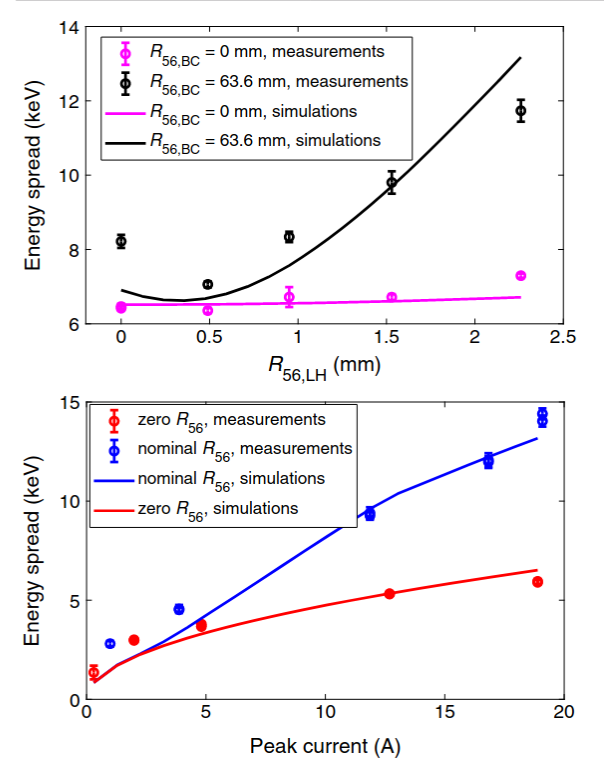
\includegraphics[width=0.58\textwidth]{figures/presentation_only/energy_spread_pratt.png}
        \end{center}
            % \caption{Varying mesh size.}
            \label{fig:meshsize_test_VICO}
    \end{figure}
\end{frame}

 \begin{frame}[allowframebreaks]
     \frametitle{References}
     \bibliography{references.bib}
 \end{frame}

\end{document}
